% 2007 年广东卷理科第 12 题：n 棱锥示意图（图中按五棱锥绘制）。
%   顶点 S 与底面五边形 A—B—C—D—E 相连；被遮挡的侧棱 S—E 与
%   底面后侧两条边画虚线。
% 来源 PDF：gaokaomath-src/普通高考/2007/2007广东理.pdf
% SHA-256：655db04340f14b909d7f248531436d45dd8cbd71e69aca976c3bd2d1e568ceed
% 原页：2007广东理.pdf 第 1 页（A3 三栏）第 3 栏，书页码 371。
% 重绘依据：按原页棱锥的顶点位置、虚实线与底面透视重绘。
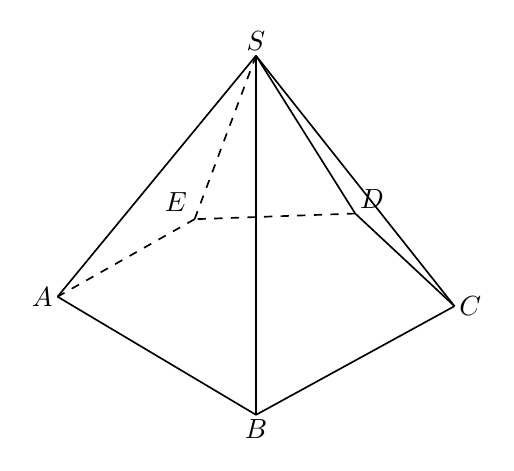
\begin{tikzpicture}[scale=1.2, semithick,
  every node/.style={inner sep=1.5pt}]

  \coordinate (S)  at (0,2.45);
  \coordinate (A)  at (-2.1,-0.10);
  \coordinate (B)  at (0,-1.35);
  \coordinate (C)  at (2.1,-0.20);
  \coordinate (D)  at (1.05,0.78);
  \coordinate (E)  at (-0.65,0.72);

  % 可见的侧棱
  \draw (S) -- (A);
  \draw (S) -- (B);
  \draw (S) -- (C);
  \draw (S) -- (D);
  % 被遮挡的侧棱
  \draw[dashed] (S) -- (E);

  % 可见的底边
  \draw (A) -- (B);
  \draw (B) -- (C);
  \draw (C) -- (D);
  % 被遮挡的底边
  \draw[dashed] (D) -- (E);
  \draw[dashed] (E) -- (A);

  \node[above] at (S) {$S$};
  \node[left]  at (A) {$A$};
  \node[below] at (B) {$B$};
  \node[right] at (C) {$C$};
  \node[above right] at (D) {$D$};
  \node[above left=1pt] at (E) {$E$};
\end{tikzpicture}
